\section{Narrow Passages}
The Navigation in the Narrow Space task is the task that allows the Tiago robot to move autonomously in a narrow space without needing to use the ROS Navigation Stack, which involves the move\_base stack, which is inefficient for the navigation in narrow spaces. We implemented a method that is divided into three parts:
\begin{itemize}
    \item in a first one we have the construction of a binary image from the data provided by listening to the topic \('/scan'\);
    \item then on the obtained image we applied some Morphological operators that help in the detection of lines using the Hough Transform;
    \item finally we used two methods to refine the lines and clustered them into two distinct clusters representing the walls of the corridor in front of the Tiago robot.
\end{itemize}
\subsection{Construction of the image}
The first step of the Navigation in a Narrow Space task is the construction of an image from the data provided by reading the \(sensor\_msgs/LaserScan\) message, subscribing to the topic \('/scan'\). In order to construct such an image, some formulas are required to change from angles in radians and distances in meters to true integer x,y coordinates.
First, we rotated the reference system of the Tiago robot by \(\pi/2\) so that the y-axis and x-axis are oriented correctly, as shown in the figure below:
\begin{center}
    \begin{figure}[H]
        \begin{minipage}{0.5\textwidth}
        \centering
        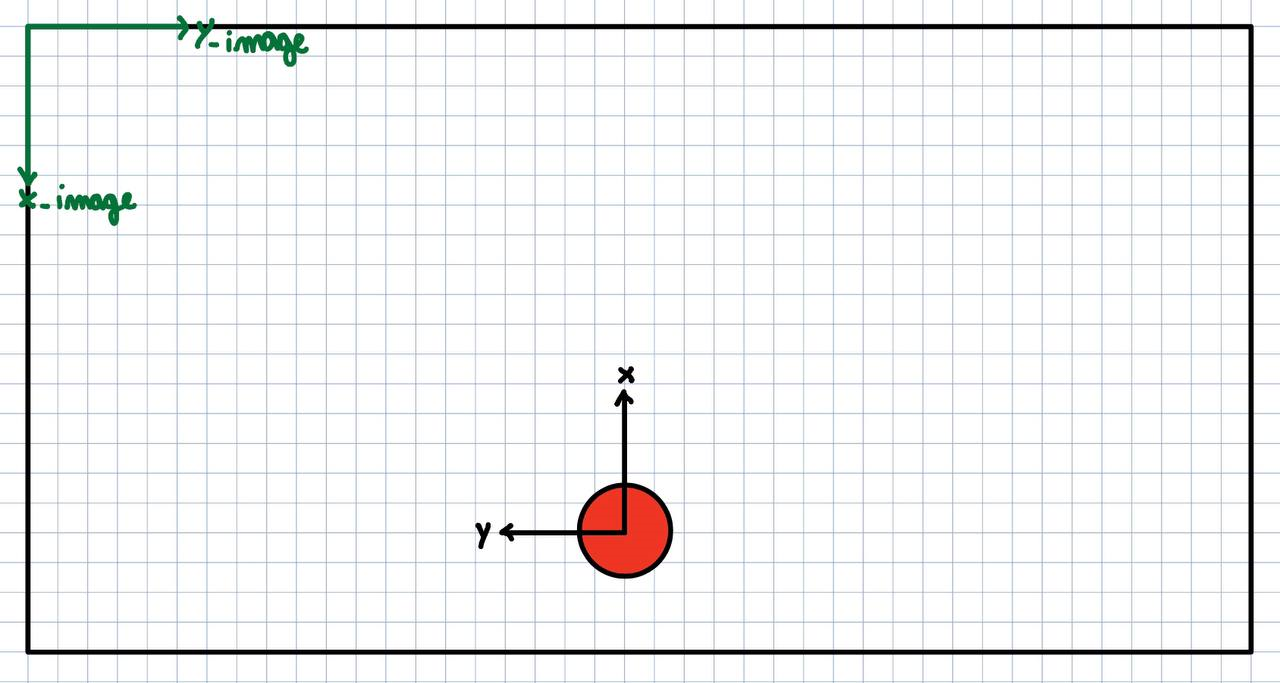
\includegraphics[scale=0.20]{images/narrowSpace/old.png}
        \captionof{figure}{Old reference frame}
    \end{minipage}
    \begin{minipage}{0.5\textwidth}
        \centering
        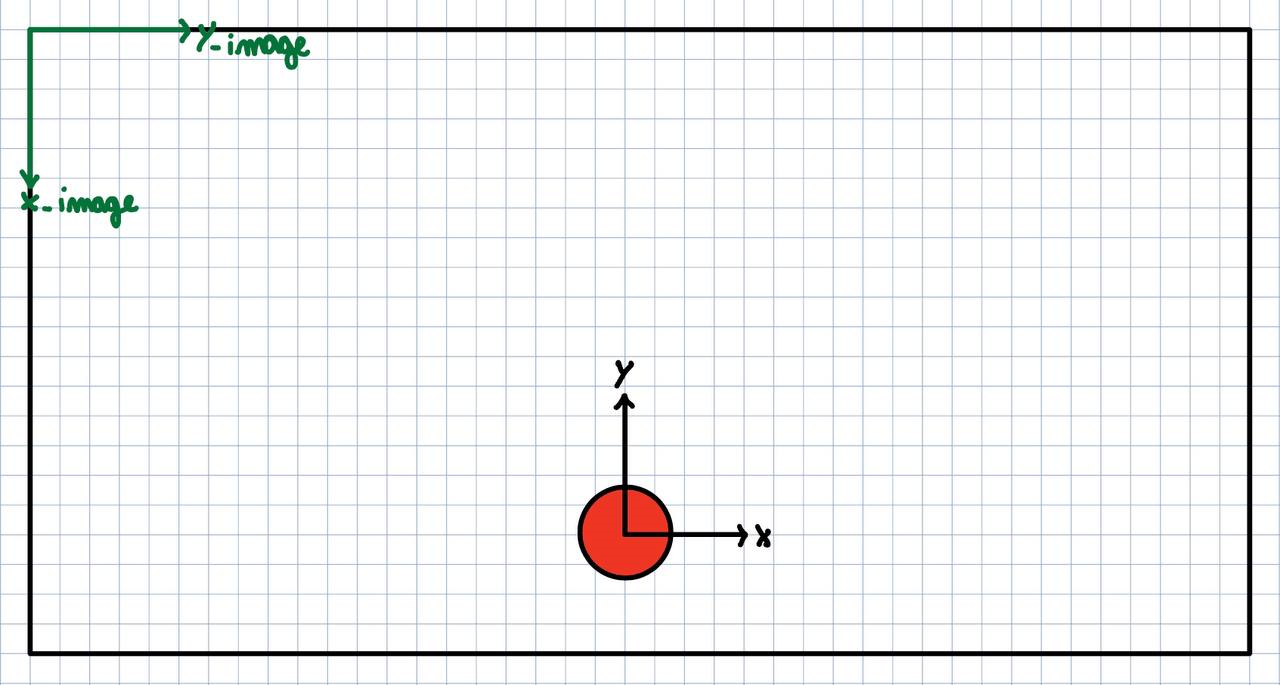
\includegraphics[scale=0.20]{images/narrowSpace/new.png}
        \captionof{figure}{New reference frame}
    \end{minipage}
    \end{figure}            
\end{center}
Next, we calculated useful quantities to start processing the laser scan data and then obtain integer coordinates in x and y; the formulas used are as follows: 
\begin{itemize}
    \item \(N_{Rows} = {\frac{(angleMin + \pi/2)}{angleIncrement}}\), to get the number of rows of the image that represent the scan of the laser;
    \item \(N_{Cols} = \floor*{\frac{\pi}{angleIncrement}}\), to get the number of columns of the image that represent the scan of the laser;
    \item \(W_{Pixel} = \frac{2 * rangeMax}{N_{Cols}}\), to get the width of a pixel of the image that represent the scan of the laser;
    \item \(H_{Pixel} = \frac{rangeMax + (rangeMax*\sin(angleMin))}{N_{Rows}}\), to get the height of a pixel of the image that represent the scan of the laser;
    \item \(X_{RawImage} = rangeMax + \rho * \sin(\theta)\), to get the 'x' float coordinate in the image reference frame of a point detected by the laser;
    \item \(Y_{RawImage} = rangeMax + \rho * \cos(\theta)\), to get the 'y' float coordinate in the image reference frame of a point detected by the laser;
    \item \(X_{Image} = \floor*{\frac{XRawImage}{H_{Pixel}}}\), to get the 'x' coordinate in the image reference frame of a point detected by the laser;
    \item \(Y_{Image} = \floor*{\frac{YRawImage}{W_{Pixel}}}\), to get the 'y' coordinate in the image reference frame of a point detected by the laser;
\end{itemize}
where 
\begin{itemize}
    \item \(angleMin = angle\_min + \pi/2\) with \(angle\_min\) that is a field of \(sensor\_msgs/LaserScan\) message, which represent the start angle of the scan [rad];
    \item angleIncrement: is the field \(angle\_increment\) of \(sensor\_msgs/LaserScan\) message, which represent the angular distance between measurements [rad];
    \item rangeMax: is the field \(range\_max\) of \(sensor\_msgs/LaserScan\) message, which represent the maximum range value [m];
    \item \(\rho\) : is the distance obtained from reading each i-th scan from \(sensor\_msgs/LaserScan\) message;
    \item \(\theta\) : is the angle obtained from \(angleMin + (angleIncrement * (i-th\_scan))\);
\end{itemize}
In order to have a visual proof of the quantities listed above, we show the following image that summarises them graphically:
\begin{center}
    \begin{figure}[H]
        \begin{minipage}{1.0\textwidth}
            \centering
                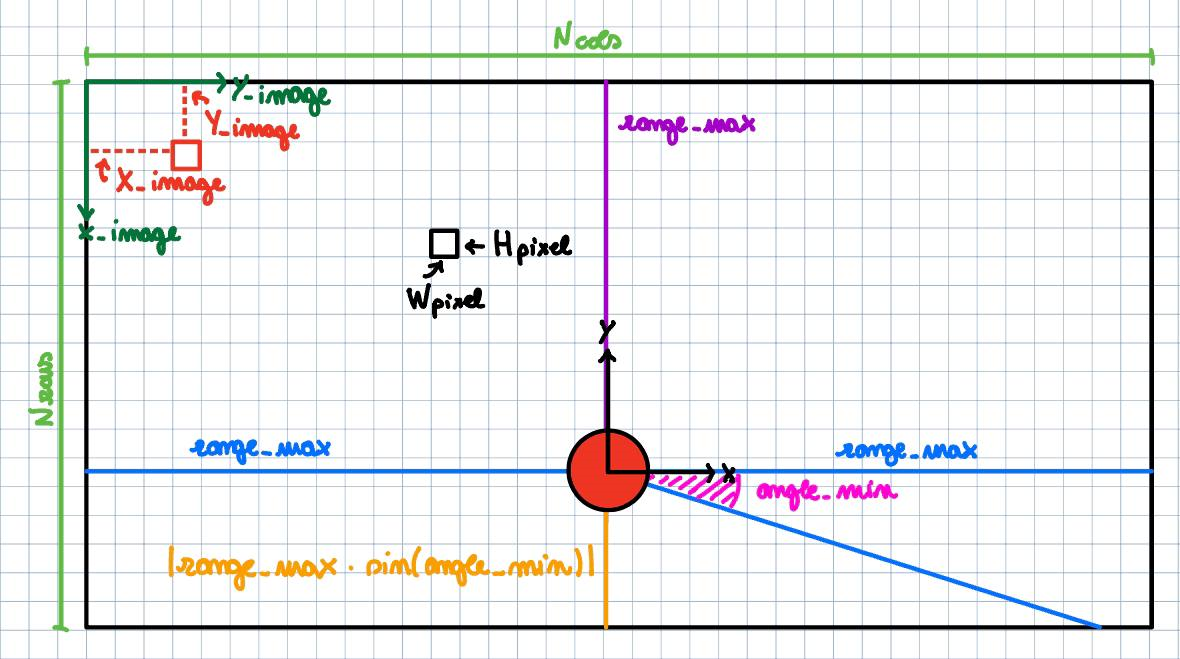
\includegraphics[scale=0.45]{images/narrowSpace/formulas.png}
            \caption{Visual proof of the quantities listed above}
        \end{minipage}
    \end{figure}            
\end{center}
The image is then constructed in such a way that each scan provided by the \(sensor\_msgs/LaserScan\) message corresponds to a white pixel in a completely black image. The result obtained is as follows:
\begin{center}
    \begin{figure}[H]
        \begin{minipage}{1.0\textwidth}
            \centering
                
\includegraphics[scale=0.70]{images/narrowSpace/initialImage.png}
            \caption{The Built Image}
        \end{minipage}
    \end{figure}            
\end{center}
\subsection{Morphological operators and Hough Transform}
The second step of the Navigation in the Narrow Space task requires the application of morphological operators such as dilation and erosion because they allow the application of a structuring element to the input image in order to shrinks or to expands the image pixels. In this case, we applied a dilation with a rect structuring element of parameters (2,25) to the input image and then an erosion with an equal structuring element of parameters (1,35) in order to shrinks better the image pixels. 
After this post-processing of the image pixels, we applied the probabilistic Hough transform with this parameters:
\begin{itemize}
    \item rho = 1;
    \item theta = \(\pi/180\); 
    \item threshold = 1;
    \item minLineLength = 8.0;
\end{itemize}
The result image obtained is the following:
\begin{center}
        \begin{figure}[H]
            \begin{minipage}{1.0\textwidth}
                \centering
                    
\includegraphics[scale=0.70]{images/narrowSpace/houghImage.png}
                \caption{The Image After Hough Transform}
            \end{minipage}
        \end{figure}            
\end{center}
\subsection{Refining and clustering the lines}
The third and last step of the Navigation in the Narrow Space task involves the use of a first clustering method to divide the detected lines into two distinct groups; this method is OpenCV's 'partition' function, which requires the specification of a predicate to perform the division; we chose a predicate that predicted that a line would belong to the cluster if it was less than a certain distance that we specified as a threshold. 
After this step we created a function that merged the lines belonging to the same cluster into two distinct lines, one per cluster, based on the average of the x,y coordinates of the points defining the single line, and then another function that refined them by considering the line with the major y coordinates, and stretching the one that was minor by looking to y coordinates, and viceversa. 
This is our final result:
\begin{center}
        \begin{figure}[H]
            \begin{minipage}{1.0\textwidth}
                \centering
                    
\includegraphics[scale=0.70]{images/narrowSpace/finalImage.png}
                \caption{The Final Image}
            \end{minipage}
        \end{figure}            
\end{center}